\subsection{MSER - \emph{Maximal Stable Extremal Regions}}

O detector MSER � composto por regi�es de todos os pixels conectados
considerando um \emph{threshold}. Em outras palavras, as regi�es selecionadas
s�o padr�es que n�o mudam e que a binariza��o local � est�vel ao longo de uma
faixa de \emph{thresholds}. Podemos fazer uma
analogia com o processo de forma��o de po�as de �gua para compreendermos como
s�o formadas as regi�es MSER, que s�o descritas em imagens em tons de cinza
representados pela fun��o $I: \Omega \rightarrow [0\ldots255] $ em que $\Omega =
[1 \ldots W]\times[1 \ldots H] $. O m�todo garante a localiza��o de objetos que
est�o mais pr�ximos de nossa realidade como pode ser observada na
Figura~\ref{fig:mserregion} \cite{MSER}.

 \begin{figure}[H]
\centering
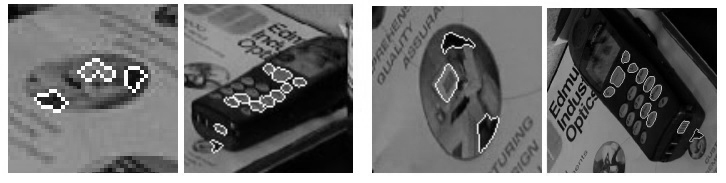
\includegraphics[scale=0.5]{images/mserregion}
\caption{Regi�es MSER. Fonte \cite{MSER}}
\label{fig:mserregion}
\end{figure}

Selecionado um \emph{threshold} de intensidades, a Figura � dividida em dois
grupos, P(pretos) e B(brancos). � observada que a quantidade de regi�es varia
dependendo do \emph{threshold} aplicado, de 0 a 255.
A �rea de cada componente conectado � ent�o armazenada como uma fun��o. Dentre
as regi�es, as mais est�veis s�o selecionadas analisando as fun��es para as quais
cada regi�o em potencial mantem seu estado com a mesma fun��o independente da
varia��o de \emph{threshold}. As regi�es ``m�ximamente est�veis'' s�o chamadas
regi�es MSER, que mudaram apenas em tamanho variando-se pelo menos alguns n�veis
de \emph{threshold}.



